\documentclass[10.5pt,a4paper]{book}

\input{"Préambule.tex"}
\usepackage{tikz}			%for TikZ graphics
\usepackage{tikz-3dplot} %for tikz-3dplot functionality
\usepackage{tkz-euclide}
\usepackage{booktabs}
\usetikzlibrary{babel}


\tikzset{elliparc/.style args={#1:#2:#3}{%
insert path={++(#1:#3) arc (#1:#2:#3)}}}

\fancyhead[L]{Guillaume Pronost}
\fancyhead[R]{1AP - Cinématique du point}%{\AdvanceDate[1]\today}

\hypersetup{
    pdftitle={Cinématique du Point}, 
	pdfauthor = {Guillaume Pronost}	
}

%\pagestyle{empty}
\definecolor{vert}{rgb}{0.0, 0.5, 0.0}
\definecolor{babyblue}{rgb}{0.54, 0.81, 0.94}
\usepackage{chemformula}
\usetikzlibrary{positioning,tikzmark}
\DeclareSIUnit\atm{atm}
\sisetup{inter-unit-product = \ensuremath{{}\cdot{}}}

\begin{document}
\setlength\intextsep{0pt}
\chapter{Cinématique du Point Matériel}

\vspace{-3ex}

\begin{flushright}

\textit{\og La vitesse n'a jamais tué personne.\\ 
 Se retrouver brusquement immobile, c'est ça qui vous tue.\fg}

- Jeremy Clarkson, \textit{Top Gear}
\end{flushright}

\vspace{2ex}

La cinématique est une branche de la mécanique qui exprime sous forme mathématique le mouvement des corps.\\
La cinématique du point constitue l’étude du mouvement d’un point indépendamment des causes qui ont engendré ce mouvement.

\begin{boite}[Point matériel]
Il arrive souvent que l'on puisse décrire et prédire le mouvement d'un objet par les lois de la dynamique, en associant l'objet à un unique point géométrique auquel on attribue la masse $m$ de l'objet. C'est ce qu'on appelle un \emph{\textbf{point matériel}}.\\
Ce point matériel constitue un \emph{modèle} de l'objet étudié. Il s'agit donc d'une approximation permettant une application simple de lois physiques sur cet objet. La modélisation du comportement de l'objet sous la forme d'un point matériel constitue une approximation de son comportement réel.
\end{boite}

\section{Rappels sur les vecteurs et les espaces vectoriels}

\begin{boite}[Comparaison des vecteurs]
Deux vecteurs non nuls $\vv u$ et $\vv v$ sont \emph{\textbf{colinéaires}} si et seulement si il existe un nombre réel $k$ tel que $\vv v = k*\vv u$.
Autrement dit, deux vecteurs sont colinéaires si l’un est un multiple de l’autre. \\

Le \emph{\textbf{produit scalaire}} de deux vecteurs $\vv u$ et $\vv v$ peut être défini comme $\vv u .\vv v = \left|\left|\vv u\right|\right| \left|\left|\vv v\right|\right| \cos{\theta}$, où $\theta$ est l’angle formé entre $\vv u$ et $\vv v$\\

Deux vecteurs non nuls $\vv u$ et $\vv v$ sont \emph{\textbf{orthogonaux}} si et seulement si leur produit scalaire est nul : $\vv u .\vv v = 0$
\end{boite}

\begin{boite}[Base d'un espace vectoriel]
Soit $E$ un espace vectoriel.\\

Une famille de vecteurs $F$ = ($\vv i_1$, $\vv i_2$, ... $\vv i_n$) de $E$ est dite \emph{libre} et ses vecteurs sont dit liénairements indépendants, lorsque
\begin{align*}
\forall \ \lambda_1,\ \lambda_2,\ ...,\ \lambda_n \in E,\ \lambda_1 \vv i_1 + \lambda_2 \vv i_2 + ... + \lambda_n \vv i_n = \vv 0 \implies \lambda_1= \lambda_2= ...=\lambda_n = 0
\end{align*}
Une famille qui n'est pas libre est dite \emph{liée}.\\

Une famille de vecteurs $F$ = ($\vv i_1$, $\vv i_2$, ... $\vv i_n$) de $E$ est dite \emph{génératrice} lorsque tout vecteur $\vv v \in E$ est combinaison des vecteurs de $F$.\\

Une famille de vecteurs $F$ = ($\vv i_1$, $\vv i_2$, ... $\vv i_n$) de $E$ est dite \emph{\textbf{base}} de $E$ lorsque qu'elle est libre et génératrice.
\end{boite}

\begin{boite}[Repère]
Soit $E$ un espace vectoriel de dimension $n$, $A$ un espace affine sur $E$. Soit ($\vv i_1$, $\vv i_2$, ... $\vv i_n$) une base de $E$ et $M$ un point de l'espace affine $A$. Alors l'ensemble ($A$, $\vv i_1$, $\vv i_2$, ... $\vv i_n$) constitue un \emph{\textbf{repère}} de $E$.
\end{boite}

\begin{boite}[Repère orthonormé direct en dimension 2 et 3]
Dans ce chapitre et les suivants, on s'interessera uniquement à des espaces de dimension 2 (problème plan) et de dimension 3 (problème en 3D). Dans ce contexte, les différents repères utilisés seront toujours des repères orthonormés directs.\\

Un repère ($A$, $\vv i_1$, ... $\vv i_n$) est dit \emph{\textbf{orthonormé}} si tout les vecteurs ($\vv i_1$, ... $\vv i_n$) composant ce repère sont des vecteurs \emph{\textbf{unitaires}}, c'est-à-dire qu'ils sont de norme 1 : 
\begin{align*}
 \left|\left|\vv i_1\right|\right|= ... =\left|\left|\vv i_n\right|\right|= 1
\end{align*}
Un repère ($A$, $\vv i_1$, ... $\vv i_n$) de dimension 2 ou 3 est dit \emph{\textbf{direct}} si il respecte la règle dite du "bonhomme d'Ampère" ou de la "main droite". Dans le cas contraire, le repère est dit \emph{\textbf{indirect}}.
\end{boite}

\section{Repérage d'un point matériel}

\begin{boite}[Référentiel]
Pour commence à discuter du mouvement d'un corps ou d'un point, il est nécessaire de définir par rapport à quoi le mouvement sera mesuré.\\

Un \emph{\textbf{référentiel}} est un solide servant de référence pour décrire le mouvement des objets. Les vitesses et accélérations sont définies par rapport à ce référentiel.\\

Sauf indication contraire, nous utiliserons le référentiel terrestre.\\

Exemples de référentiels :
\begin{itemize}
    \item Le référentiel héliocentrique (ou référentiel de Kepler)
    \item Le référentiel géocentrique
    \item Le référentiel terrestre
\end{itemize}
Nous supposerons qu’il existe un temps absolu : deux observateurs en mouvement relatifs peuvent attribuer les mêmes dates aux mêmes événements.
\end{boite}

\begin{boite}[Trajectoire d'un point]
On appelle \emph{\textbf{trajectoire}} d'un point, dans un référentiel, l'ensemble des positions successives occupées par ce point au cours du temps.\\

Soit $O$ un point particulier du référentiel et $M$ la position du point matériel. La fonction $\overrightarrow{OM}(t)$ donne la position du point matériel $M$ au cours du temps $t$. On la nomme \emph{\textbf{équation horaire}}.\\

Déterminer cette fonction $\overrightarrow{OM}(t)$ représente l'objectif principal de la mécanique du point.
\end{boite}

\newpage
\subsection{Position d'un point en 2 dimensions}

On place un observateur à un point $O$ du référentiel, nommé \emph{\textbf{origine}}. On cherche à exprimer la position d'un point matériel $M$ par rapport à un repère orthonormé direct ($O$, $\vv u_1$, $\vv u_2$).

\begin{boite}[Coordonnées cartésiennes]

\begin{minipage}{.5\textwidth}
\begin{tikzpicture}[>=Latex,scale=2.0]
%\tkzDefPoint(0,0){O} ;
%\tkzDefPoint(3,0){vx} ;
%\tkzDefPoint(0,2){vy} ;
%\tkzLabelPoints[left](O) ;
%\tkzLabelPoint[above](vx){$\vv x$} ;
%\tkzLabelPoint[above left](vy){$\vv y$} ;

\tkzDefPoint[label={left:$O$}](0,0){O}
\tkzDefPoint[label={above:$\vv x$}](3,0){vx}
\tkzDefPoint[label={above left:$\vv y$}](0,2){vy}
\tkzDrawSegment[->](O,vx) ;
\tkzDrawSegment[->](O,vy);

\tkzDefPoint(1,0){ux} ;
\tkzDefPoint(0,1){uy} ;
\draw (1,0.4) node[red] {$\vv u_x$} ;
\tkzDrawSegment[red,->,thick](O,ux) ;
\draw (-0.4,1) node[red] {$\vv u_y$} ;
\tkzDrawSegment[red,->,thick](O,uy) ;

\tkzDefPoint(1.8,1.3){M} ;
\tkzDrawSegment(O,M) ;
\tkzDrawPoint(M);
\tkzLabelPoints[above right](M) ;
\tkzDefPointBy[projection=onto O--vx](M) \tkzGetPoint{xM}
\tkzDefPointBy[projection=onto O--vy](M) \tkzGetPoint{yM}
\tkzLabelPoint[below](xM){$x$} ;
\tkzLabelPoint[above left](yM){$y$} ;
\tkzDrawSegment[dashed](M,xM) ;
\tkzDrawSegment[dashed](M,yM) ;

\end{tikzpicture}
\end{minipage}
\hfill
\begin{minipage}{.48\textwidth}
\begin{flushleft}
Le point $M$ est repéré par les coordonnées cartésiennes ($x$, $y$)
\begin{align*}
 \vv{OM} &= x \vv u_x + y \vv u_y \\ x, y \ &\in \ ]-\infty, +\infty[
\end{align*}
\end{flushleft} 
\end{minipage}

Le repère associé aux coordonnées cartésiennes permet de décrire les coordonnées d’un point $M(x, y)$ et les composantes d’un vecteur $\vv V(V_x, V_y)$ sur la base ($\vv u_x$, $\vv u_y$).\\

Dans la suite, le référentiel $R_c$ associé aux coordonnées cartésiennes sera considéré comme fixe.
\end{boite}

Il se peut que les coordonnées cartésiennes ne soient pas les plus commodes pour décrire la position d'un point matériel. C'est notamment le cas lorsqu'on veut décrire un mouvement de rotation, tel qu'un mouvement sur une sphère ou un cylindre.

\begin{boite}[Coordonnées polaires]

\begin{minipage}{.5\textwidth}
\begin{tikzpicture}[>=Latex,scale=2.0]
%\tkzDefPoint(0,0){O} ;
%\tkzDefPoint(3,0){vx} ;
%\tkzDefPoint(0,2){vy} ;
%\tkzLabelPoints[left](O) ;
%\tkzLabelPoint[above](vx){$\vv x$} ;
%\tkzLabelPoint[above left](vy){$\vv y$} ;

\tkzDefPoint[label={left:$O$}](0,0){O}
\tkzDefPoint[label={above:$\vv x$}](3,0){vx}
\tkzDefPoint[label={above left:$\vv y$}](0,2){vy}
\tkzDrawSegment[->](O,vx) ;
\tkzDrawSegment[->](O,vy);

\tkzDefPoint(1.8,1.3){M} ;
\tkzDrawSegment(O,M) ;
\tkzDrawPoint(M);
\tkzLabelSegment[above,pos=.6](O,M){$r$}
\tkzLabelPoints[below right](M) ;

\tkzDefPointWith[linear,K=2](O,M) \tkzGetPoint{M2}
\tkzDefPointWith[linear normed](M,M2) \tkzGetPoint{ur}
\tkzDefPointWith[orthogonal normed](M,ur) \tkzGetPoint{utheta}
\tkzDrawSegment[red,->,thick](M,ur);
\tkzDrawSegment[red,->,thick](M,utheta) ;
\tkzLabelPoint[below right, red](ur){$\vv u_r$} ;
\tkzLabelPoint[above, red](utheta){$\vv u_\theta$} ;

\tkzMarkAngle[mark=none,size=1cm,->,color=red](vx,O,M) ;
\tkzLabelAngle[color=red,xshift=.3cm,yshift=.1cm](vx,O,M){$\theta$} ;


\end{tikzpicture}
\end{minipage}
\hfill
\begin{minipage}{.48\textwidth}
\begin{flushleft}
Le point $M$ est repéré par les coordonnées polaires ($r$, $\theta$)
\begin{align*}
\vv{OM} &= r \vv u_r  \\ r \ &\in \ [0, +\infty[ \\ \theta \ &\in \ [0, 2\pi[
\end{align*}
\end{flushleft} 
\end{minipage}

Le repère associé aux coordonnées polaires permet de décrire les coordonnées d’un point $M ( r, \theta)$ et les composantes d’un vecteur $\vv V(V_r, V_\theta)$ sur la base ($\vv u_r$, $\vv u_\theta$).\\

Il est important de remarquer que la base dépend de la coordonnée $\theta$ du point $M$.\\

En général, les coordonnées cartésiennes sont associées au référentiel terrestre, considéré comme \emph{\textbf{galiléen}}. Les coordonnées polaires, quant à elles, sont particulièrement adaptées à l’étude des mouvements de rotation. La base est souvent appelée \emph{\textbf{base mobile}}. On dit qu’elle est associée au référentiel tournant $R_T$.

\begin{theoreme}[Changement de base]
On s'interesse à une base fixe ($\vv u_x$, $\vv u_y$) et à une base mobile ($\vv u_r$, $\vv u_\theta$).
Tout les vecteurs des bases sont unitaires. On a donc : 
\begin{align*}
\left|\left|\vv u_x\right|\right|=\left|\left|\vv u_y\right|\right|=\left|\left|\vv u_r\right|\right|=\left|\left|\vv u_\theta\right|\right|=1
\end{align*}

\begin{minipage}{.38\textwidth}
\begin{flushleft}
\begin{align*}
\vv u_r &= \vv u_{r_x} + \vv u_{r_y} \\
\vv u_r &= \cos{\theta}\vv u_x + \sin{\theta}\vv u_y\\
&\\
\vv u_\theta &= \vv u_{\theta_x} + \vv u_{\theta_y} \\
\vv u_\theta &= -\sin{\theta}\vv u_x + \cos{\theta}\vv u_y
\end{align*}
\end{flushleft} 
\end{minipage}
\hfill
\begin{minipage}{.6\textwidth}
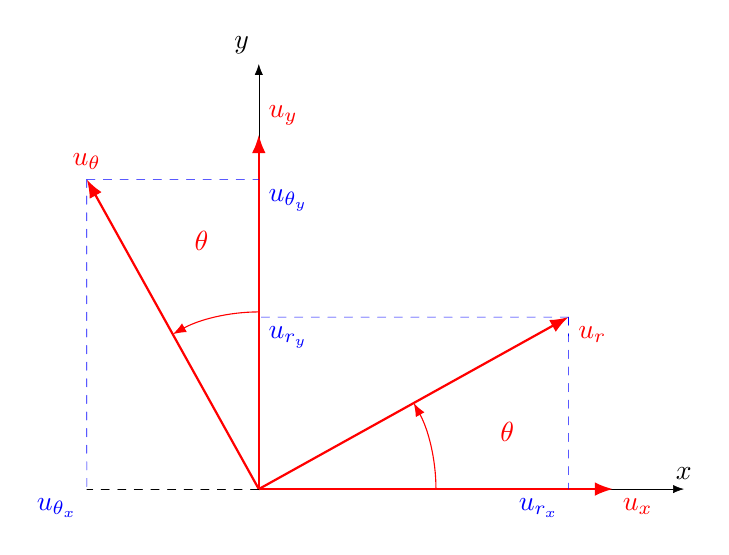
\begin{tikzpicture}[>=Latex,scale=4.5]
%\tkzDefPoint(0,0){O} ;
%\tkzDefPoint(3,0){vx} ;
%\tkzDefPoint(0,2){vy} ;
%\tkzLabelPoints[left](O) ;
%\tkzLabelPoint[above](vx){$\vv x$} ;
%\tkzLabelPoint[above left](vy){$\vv y$} ;

\tkzDefPoint(0,0){O}
\tkzDefPoint[label={above:$\vv x$}](1.2,0){vx}
\tkzDefPoint[label={above left:$\vv y$}](0,1.2){vy}
\tkzDrawSegment[->](O,vx) ;
\tkzDrawSegment[->](O,vy);

\tkzDefPoint(1,0){ux} ;
\tkzDefPoint(0,1){uy} ;
\tkzDrawSegment[red,->,thick](O,ux) ;
\tkzDrawSegment[red,->,thick](O,uy) ;
\tkzLabelPoint[below right, red](ux){$\vv u_x$} ;
\tkzLabelPoint[above right, red](uy){$\vv u_y$} ;

\tkzDefPoint(1.8,1){M} ;

\tkzDefPointWith[linear normed](O,M) \tkzGetPoint{ur}
\tkzDefPointWith[orthogonal normed](O,ur) \tkzGetPoint{utheta}
\tkzDrawSegment[red,->,thick](O,ur);
\tkzDrawSegment[red,->,thick](O,utheta) ;
\tkzLabelPoint[below right, red](ur){$\vv u_r$} ;
\tkzLabelPoint[above, red](utheta){$\vv u_\theta$} ;

\tkzMarkAngle[mark=none,size=.5cm,->,color=red](vx,O,ur) ;
\tkzLabelAngle[color=red,xshift=-1.2cm,yshift=-.4cm](vx,O,ur){$\theta$} ;
\tkzMarkAngle[mark=none,size=.5cm,->,color=red](vy,O,utheta) ;
\tkzLabelAngle[color=red,xshift=.4cm,yshift=-1.2cm](vy,O,utheta){$\theta$} ;

\tkzDefPointBy[projection=onto O--vx](ur) \tkzGetPoint{urx}
\tkzDefPointBy[projection=onto O--vy](ur) \tkzGetPoint{ury}
\tkzLabelPoint[below left, blue](urx){$\vv u_{r_x}$} ;
\tkzLabelPoint[below right, blue](ury){$\vv u_{r_y}$} ;
\tkzDrawSegment[dashed, blue](ur,urx) ;
\tkzDrawSegment[dashed, blue](ur,ury) ;

\tkzDefPointBy[projection=onto O--vx](utheta) \tkzGetPoint{utx}
\tkzDefPointBy[projection=onto O--vy](utheta) \tkzGetPoint{uty}
\tkzLabelPoint[below left, blue](utx){$\vv u_{\theta_x}$} ;
\tkzLabelPoint[below right, blue](uty){$\vv u_{\theta_y}$} ;
\tkzDrawSegment[dashed, blue](utheta,utx) ;
\tkzDrawSegment[dashed, blue](utheta,uty) ;
\tkzDrawSegment[dashed](O,utx) ;
\end{tikzpicture}
\end{minipage}

\begin{minipage}{.38\textwidth}
\begin{flushleft}
\begin{align*}
\vv u_x &= \vv u_{x_r} + \vv u_{x_\theta} \\
\vv u_x &= \cos{\theta}\vv u_r - \sin{\theta}\vv u_\theta\\
&\\
\vv u_y &= \vv u_{y_r} + \vv u_{y_\theta} \\
\vv u_y &= \sin{\theta}\vv u_r + \cos{\theta}\vv u_\theta
\end{align*}
\end{flushleft} 
\end{minipage}
\hfill
\begin{minipage}{.6\textwidth}
\begin{tikzpicture}[>=Latex,scale=4.5]
%\tkzDefPoint(0,0){O} ;
%\tkzDefPoint(3,0){vx} ;
%\tkzDefPoint(0,2){vy} ;
%\tkzLabelPoints[left](O) ;
%\tkzLabelPoint[above](vx){$\vv x$} ;
%\tkzLabelPoint[above left](vy){$\vv y$} ;

\tkzDefPoint(0,0){O}
\tkzDefPoint[label={above:$\vv x$}](1.2,0){vx}
\tkzDefPoint[label={above left:$\vv y$}](0,1.2){vy}
\tkzDrawSegment[->](O,vx) ;
\tkzDrawSegment[->](O,vy);

\tkzDefPoint(1,0){ux} ;
\tkzDefPoint(0,1){uy} ;
\tkzDrawSegment[red,->,thick](O,ux) ;
\tkzDrawSegment[red,->,thick](O,uy) ;
\tkzLabelPoint[below right, red](ux){$\vv u_x$} ;
\tkzLabelPoint[above right, red](uy){$\vv u_y$} ;

\tkzDefPoint(1.8,1){M} ;

\tkzDefPointWith[linear normed](O,M) \tkzGetPoint{ur}
\tkzDefPointWith[orthogonal normed](O,ur) \tkzGetPoint{utheta}
\tkzDrawSegment[red,->,thick](O,ur);
\tkzDrawSegment[red,->,thick](O,utheta) ;
\tkzLabelPoint[below right, red](ur){$\vv u_r$} ;
\tkzLabelPoint[above, red](utheta){$\vv u_\theta$} ;

\tkzMarkAngle[mark=none,size=.5cm,->,color=red](vx,O,ur) ;
\tkzLabelAngle[color=red,xshift=-1.2cm,yshift=-.4cm](vx,O,ur){$\theta$} ;
\tkzMarkAngle[mark=none,size=.5cm,->,color=red](vy,O,utheta) ;
\tkzLabelAngle[color=red,xshift=.4cm,yshift=-1.2cm](vy,O,utheta){$\theta$} ;

\tkzDefPointBy[projection=onto O--ur](ux) \tkzGetPoint{uxr}
\tkzDefPointBy[projection=onto O--utheta](ux) \tkzGetPoint{uxt}
\tkzLabelPoint[below left, blue](uxr){$\vv u_{x_r}$} ;
\tkzLabelPoint[below right, blue](uxt){$\vv u_{x_\theta}$} ;
\tkzDrawSegment[dashed, blue](ux,uxr) ;
\tkzDrawSegment[dashed, blue](ux,uxt) ;

\tkzDefPointBy[projection=onto O--ur](uy) \tkzGetPoint{uyr}
\tkzDefPointBy[projection=onto O--utheta](uy) \tkzGetPoint{uyt}
\tkzLabelPoint[below left, blue](uyr){$\vv u_{y_r}$} ;
\tkzLabelPoint[below right, blue](uyt){$\vv u_{y_\theta}$} ;
\tkzDrawSegment[dashed, blue](uy,uyr) ;
\tkzDrawSegment[dashed, blue](uy,uyt) ;
\tkzDrawSegment[dashed](O,uxt) ;
\end{tikzpicture}
\end{minipage}  
\end{theoreme}

On a pu voir que différents systèmes de coordonnées permettaient de représenter la position du point $M$. Ainsi :
\begin{align*}
 \overrightarrow{OM} &= x \vv u_x + y \vv u_y \\ 
 & \text{et}\\
\overrightarrow{OM} &= r \vv u_r
\end{align*}
A partir des formules de projections déterminées précedemment, il est possible d'exprimer les coordonnées cartésiennes ($x$, $y$) en fonction des coordonnées polaires ($r$, $\theta$) et inversemment. Ainsi :
\begin{equation*}
    \begin{cases}
      x &= \ r \cos{\theta}  \\
      y &= \ r \sin{\theta} 
    \end{cases}       
\end{equation*}

\end{boite}

\subsection{Position d'un point en 3 dimensions}

On place un observateur à un point $O$ du référentiel, nommé \emph{\textbf{origine}}. On cherche à exprimer la position d'un point matériel $M$ par rapport à un repère orthonormé direct ($O$, $\vv u_1$, $\vv u_2$, $\vv u_3$).

\begin{boite}[Coordonnées cartésiennes]

\begin{minipage}{.5\textwidth}
\begin{tikzpicture}[>=Latex,scale=1.8]
%\tkzDefPoint(0,0){O} ;
%\tkzDefPoint(-1,-1){x} ;
%\tkzDefPoint(2,0){y} ;
%\tkzDefPoint(0,2){z} ;
%\tkzLabelPoints[left](O) ;
%\tkzLabelPoints[below left](x) ;
%\tkzLabelPoints[above](y) ;
%\tkzLabelPoints[above left](z) ;

\tkzDefPoint[label={left:$O$}](0,0){O}
\tkzDefPoint[label={below left:$\vv x$}](-1,-1){vx}
\tkzDefPoint[label={above:$\vv y$}](2.3,0){vy}
\tkzDefPoint[label={above left:$\vv z$}](0,2){vz}
\tkzDrawSegment[->](O,vx) ;
\tkzDrawSegment[->](O,vy);
\tkzDrawSegment[->](O,vz);

\tkzDefPoint(-0.4,-0.4){ux} ;
\draw (-0.8,-0.4) node[red] {$\vv u_x$} ;
\tkzDefPoint(1,0){uy} ;
\draw (1,0.4) node[red] {$\vv u_y$} ;
\tkzDefPoint(0,1){uz} ;
\draw (-0.4,1) node[red] {$\vv u_z$} ;

\tkzDrawSegment[red,->,thick](O,ux) ;
\tkzDrawSegment[red,->,thick](O,uy) ;
\tkzDrawSegment[red,->,thick](O,uz) ;

\tkzDefPoint(1.2,1.1){M} ;
\tkzDrawSegment(O,M) ;
\tkzDrawPoint(M);
\tkzLabelPoints[above right](M) ;
\tkzDefPoint(1.2,-0.5){M'} ;
\tkzDrawSegment[dashed](O,M') ;
%\tkzLabelPoints[below right](M') ;

\tkzDefPointBy[translation=from O to vy](M') \tkzGetPoint{xM1}
\tkzInterLL(O,vx)(M',xM1) \tkzGetPoint{xM}
\tkzDefPointBy[translation=from O to vx](M') \tkzGetPoint{yM1}
\tkzInterLL(O,vy)(M',yM1) \tkzGetPoint{yM}
%\tkzDefPointBy[projection=onto O--vy](M') \tkzGetPoint{yM}
\tkzDefPointBy[translation=from O to M'](M) \tkzGetPoint{zM1}
\tkzInterLL(O,vz)(M,zM1) \tkzGetPoint{zM}

\tkzLabelPoint[below right](xM){$x$} ;
\tkzLabelPoint[above ](yM){$y$} ;
\tkzLabelPoint[above left](zM){$z$} ;
\tkzDrawSegment[dashed](M',xM) ;
\tkzDrawSegment[dashed](M',yM) ;
\tkzDrawSegment[dashed](M,zM) ;
\tkzDrawSegment[dashed](M',M) ;

\tkzMarkRightAngle[,size=.1,color=red](O,M',M)
\tkzMarkRightAngle[,size=.1,color=red](O,zM,M)

\end{tikzpicture}
\end{minipage}
\hfill
\begin{minipage}{.48\textwidth}
\begin{flushleft}
Le point $M$ est repéré par les coordonnées cartésiennes ($x$, $y$, $z$)
\begin{align*}
&\vv{OM} = x \vv u_x + y \vv u_y + z \vv u_z \\ &x, y, z \ \in \ ]-\infty, +\infty[
\end{align*}
\end{flushleft} 
\end{minipage}

Le repère associé aux coordonnées cartésiennes permet de décrire les coordonnées d’un point $M(x, y, z)$ et les composantes d’un vecteur $\vv V(V_x, V_y, V_z)$ sur la base ($\vv u_x$, $\vv u_y$, $\vv u_z$).\\

Dans la suite, le référentiel $R_c$ associé aux coordonnées cartésiennes sera considéré comme fixe.
\end{boite}

\begin{boite}[Coordonnées cylindriques]

\begin{minipage}{.5\textwidth}
\begin{tikzpicture}[>=Latex,scale=1.8]
%\tkzDefPoint(0,0){O} ;
%\tkzDefPoint(-1,-1){x} ;
%\tkzDefPoint(2,0){y} ;
%\tkzDefPoint(0,2){z} ;
%\tkzLabelPoints[left](O) ;
%\tkzLabelPoints[below left](x) ;
%\tkzLabelPoints[above](y) ;
%\tkzLabelPoints[above left](z) ;

\tkzDefPoint[label={left:$O$}](0,0){O}
\tkzDefPoint[label={below left:$\vv x$}](-1,-1){vx}
\tkzDefPoint[label={above:$\vv y$}](2.3,0){vy}
\tkzDefPoint[label={above left:$\vv z$}](0,2){vz}
\tkzDrawSegment[->](O,vx) ;
\tkzDrawSegment[->](O,vy);
\tkzDrawSegment[->](O,vz);

\tkzDefPoint(1.2,1.1){M} ;
\tkzDrawPoint(M);
\tkzDrawSegment(O,M) ;
\tkzLabelPoints[below right](M) ;
\tkzDefPoint(1.2,-0.5){M'} ;
\tkzDrawSegment[dashed](O,M') ;
%\tkzLabelPoints[below right](M') ;

\draw[thin] (0,0) [elliparc=0:360:1.75cm and .7cm];
\draw[thin] (0,1.6) [elliparc=0:360:1.75cm and .7cm];

%\tkzDefPointBy[translation=from O to vy](M') \tkzGetPoint{xM1}
%\tkzInterLL(O,vx)(M',xM1) \tkzGetPoint{xM}
%\tkzDefPointBy[translation=from O to vx](M') \tkzGetPoint{yM1}
%\tkzInterLL(O,vy)(M',yM1) \tkzGetPoint{yM}

\tkzDefPointBy[translation=from O to M'](M) \tkzGetPoint{zM1}
\tkzInterLL(O,vz)(M,zM1) \tkzGetPoint{zM}

%\tkzLabelPoint[below right](xM){$x$} ;
%\tkzLabelPoint[above ](yM){$y$} ;
%\tkzLabelPoint[above left](zM){$z$} ;
%\tkzDrawSegment[dashed](M',xM) ;
%\tkzDrawSegment[dashed](M',yM) ;
\tkzDrawSegment[dashed](M,zM) ;
\tkzLabelSegment[above,pos=.5](M,zM){$r$}
\tkzLabelSegment(O,zM){$z$}
\tkzDrawSegment[dashed](M',M) ;
\tkzMarkAngle[mark=none,size=.6cm,->,color=red](vx,O,M') ;
\tkzLabelAngle[color=red,xshift=.3cm,yshift=.1cm](vx,O,M'){$\theta$} ;

\tkzDefPointWith[linear,K=2](zM,M) \tkzGetPoint{M2}
\tkzDefPointWith[linear normed](M,M2) \tkzGetPoint{ur}
\tkzDefPointWith[colinear normed= at M](M',yM) \tkzGetPoint{utheta}
\tkzDefPointWith[colinear normed= at M](O,zM) \tkzGetPoint{uz}
\tkzDrawSegment[red,->,thick](M,ur);
\tkzDrawSegment[red,->,thick](M,utheta) ;
\tkzDrawSegment[red,->,thick](M,uz) ;
\tkzLabelPoint[below right, red](ur){$\vv u_r$} ;
\tkzLabelPoint[above, red](utheta){$\vv u_\theta$} ;
\tkzLabelPoint[above, red](uz){$\vv u_z$} ;

\tkzMarkRightAngle[,size=.1,color=red](O,M',M);
\tkzMarkRightAngle[,size=.1,color=red](O,zM,M);
\tkzMarkRightAngle[,size=.1,color=red](ur,M,utheta);
\tkzMarkRightAngle[,size=.1,color=red](uz,M,utheta);

\end{tikzpicture}
\end{minipage}
\hfill
\begin{minipage}{.48\textwidth}
\begin{flushleft}
Le point $M$ est repéré par les coordonnées cylindriques ($r$, $\theta$, $z$)
\begin{align*}
  \vv{OM} &= r \vv u_r  \\ r \ &\in \ [0, +\infty[ \\ \theta \ &\in \ [0, 2\pi[ \\ z \ &\in \ ]-\infty, +\infty[
\end{align*}
\end{flushleft}
\end{minipage}

\vspace{2mm}

On utilisera les coordonnées cylindriques dès que la distance à l’axe $O_z$ joue un rôle important dans l’exercice.\\

\textbf{Changement de système de coordonnées}\\

A partir des formules de projections déterminées précedemment, il est possible d'exprimer les coordonnées cartésiennes ($x$, $y$, $z$) en fonction des coordonnées cylindriques ($r$, $\theta$, $z$) et inversemment. Ainsi :
\begin{equation*}
    \begin{cases}
      x &= \ r \cos{\theta}  \\
      y &= \ r \sin{\theta} \\
      z &= \ z
    \end{cases}       
\end{equation*}
\end{boite}

\begin{boite}[Coordonnées sphériques]

\begin{minipage}{.5\textwidth}
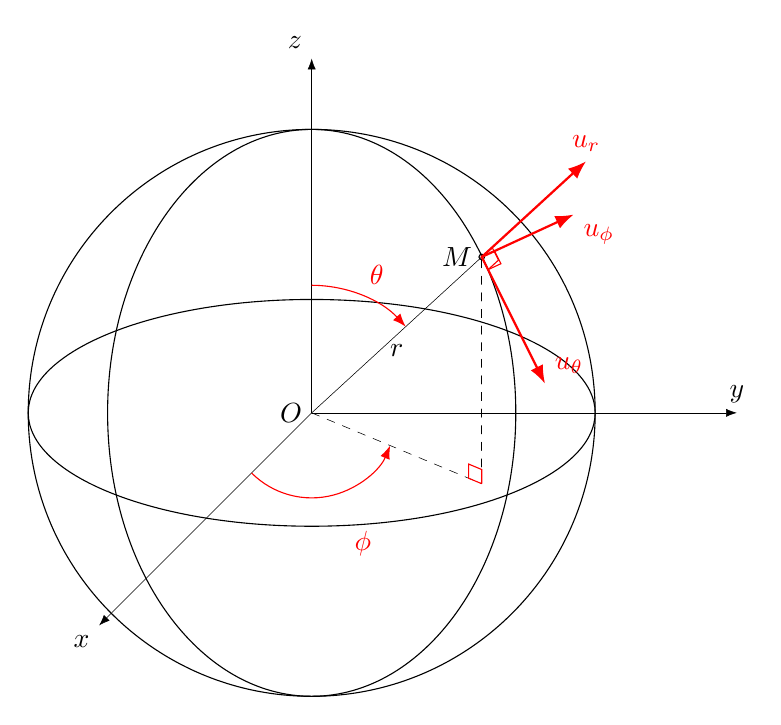
\begin{tikzpicture}[>=Latex,scale=1.8]
%\tkzDefPoint(0,0){O} ;
%\tkzDefPoint(-1,-1){x} ;
%\tkzDefPoint(2,0){y} ;
%\tkzDefPoint(0,2){z} ;
%\tkzLabelPoints[left](O) ;
%\tkzLabelPoints[below left](x) ;
%\tkzLabelPoints[above](y) ;
%\tkzLabelPoints[above left](z) ;

\tkzDefPoint[label={left:$O$}](0,0){O}
\tkzDefPoint[label={below left:$\vv x$}](-1.5,-1.5){vx}
\tkzDefPoint[label={above:$\vv y$}](3.0,0){vy}
\tkzDefPoint[label={above left:$\vv z$}](0,2.5){vz}
\tkzDrawSegment[->](O,vx) ;
\tkzDrawSegment[->](O,vy);
\tkzDrawSegment[->](O,vz);

\tkzDefPoint(1.2,1.1){M} ;
\tkzDrawPoint(M);
\tkzDrawSegment(O,M) ;
\tkzLabelPoints[left](M) ;
\tkzDefPoint(1.2,-0.5){M'} ;
\tkzDrawSegment[dashed](O,M') ;
%\tkzLabelPoints[below right](M') ;

\draw[thin] (0,0) [elliparc=0:360:2.0cm and .8cm];
\draw[thin] (0,0) [elliparc=0:360:1.44cm and 2.0cm];
\draw[thin] (0,0) [elliparc=0:360:2.0cm and 2.0cm];

%\tkzDefPointBy[translation=from O to vy](M') \tkzGetPoint{xM1}
%\tkzInterLL(O,vx)(M',xM1) \tkzGetPoint{xM}
%\tkzDefPointBy[translation=from O to vx](M') \tkzGetPoint{yM1}
%\tkzInterLL(O,vy)(M',yM1) \tkzGetPoint{yM}

\tkzDefPointBy[translation=from O to M'](M) \tkzGetPoint{zM1}
\tkzInterLL(O,vz)(M,zM1) \tkzGetPoint{zM}

%\tkzLabelPoint[below right](xM){$x$} ;
%\tkzLabelPoint[above ](yM){$y$} ;
%\tkzLabelPoint[above left](zM){$z$} ;
%\tkzDrawSegment[dashed](M',xM) ;
%\tkzDrawSegment[dashed](M',yM) ;
%\tkzDrawSegment[dashed](M,zM) ;
%\tkzLabelSegment[above,pos=.5](M,zM){$r$}
\tkzLabelSegment[below,pos=.5](O,M){$r$}
\tkzDrawSegment[dashed](M',M) ;
\tkzMarkAngle[mark=none,size=.6cm,->,color=red](vx,O,M') ;
\tkzLabelAngle[color=red,xshift=.3cm,yshift=.1cm](vx,O,M'){$\phi$} ;
\tkzMarkAngle[mark=none,size=.9cm,<-,color=red](M,O,vz) ;
\tkzLabelAngle[color=red,xshift=.1cm,yshift=.1cm](M,O,vz){$\theta$} ;

\tkzDefPointWith[linear,K=2](O,M) \tkzGetPoint{M2}
\tkzDefPointWith[linear normed](M,M2) \tkzGetPoint{ur}
\tkzDefPoint(1.85,1.4){phi} ;
\tkzDefPointWith[linear](M,phi) \tkzGetPoint{uphi}
\tkzDefPoint(1.4,0.7){theta} ;
\tkzDefPointWith[linear normed](M,theta) \tkzGetPoint{utheta}
\tkzDrawSegment[red,->,thick](M,ur);
\tkzDrawSegment[red,->,thick](M,utheta) ;
\tkzDrawSegment[red,->,thick](M,uphi) ;
\tkzLabelPoint[above, red](ur){$\vv u_r$} ;
\tkzLabelPoint[above right, red](utheta){$\vv u_\theta$} ;
\tkzLabelPoint[below right, red](uphi){$\vv u_\phi$} ;

\tkzMarkRightAngle[,size=.1,color=red](O,M',M);
\tkzMarkRightAngle[,size=.1,color=red](ur,M,utheta);
\tkzMarkRightAngle[,size=.1,color=red](uphi,M,utheta);
\end{tikzpicture}
\end{minipage}
\hfill
\begin{minipage}{.48\textwidth}
\begin{flushleft}
Le point $M$ est repéré par les coordonnées sphériques ($r$, $\theta$, $\phi$)
\begin{align*}
  \vv{OM} &= r \vv u_r  \\ r \ &\in \ [0, +\infty[ \\ \theta \ &\in \ [0, \pi[ \\ \phi \ &\in \ [0, 2\pi[
\end{align*}
\end{flushleft}
\end{minipage}

\vspace{5mm}

On utilisera les coordonnées sphériques dès que la distance $r$ au centre O joue un rôle important dans l’exercice.\\

\textbf{Changement de système de coordonnées}\\

A partir des formules de projections déterminées précedemment, il est possible d'exprimer les coordonnées cartésiennes ($x$, $y$, $z$) en fonction des coordonnées sphériques ($r$, $\theta$, $\phi$) et inversemment. Ainsi :
\begin{equation*}
    \begin{cases}
      x &= \ r \sin{\theta}\cos{\phi}  \\
      y &= \ r \sin{\theta}\sin{\phi} \\
      z &= \ r \cos{\theta}
    \end{cases}       
\end{equation*}
\end{boite}

\section{Vitesse d'un point}

En cinématique, la vitesse peut être définie comme est une grandeur qui mesure pour un mouvement, le rapport de la distance parcourue au temps écoulé.\\

Soit $M$ la position d'un mobile à un instant $t$. Soit $R$ un référentiel et $O$ un point fixe de ce référentiel.\\
On note $\vv v(M_{/R})$ le vecteur vitesse du mobile par rapport au référentiel $R$.\\
On peut exprimer alors cette vitesse :
\begin{align*}
    \tikz[baseline]{
        \node[fill=red!20,anchor=base,rounded corners]
        {$\vv v(M_{/R})=\left(\dfrac{d(\vv{OM})}{dt}\right)_{/R}$};
    } 
\end{align*}

Sauf mention contraire le référentiel $R_c$ par rapport auquel nous calculerons la vitesse sera celui associé aux coordonnées cartésiennes. \\
Dans ce référentiel $R_c$, l'origine $O$ ainsi que la base ($\vv u_x$, $\vv u_y$, $\vv u_z$) sont fixes.

\begin{boite}[Expression de la vitesse en coordonnées cartésiennes]
Soit ($\vv u_x$, $\vv u_y$, $\vv u_z$) la base des coordonnées cartésiennes.
\begin{align*}
    &\vv v(M_{/R_c})=\left(\frac{d(\vv{OM})}{dt}\right)_{/Rc} \ \ \text{avec} \ \ \vv{OM} = x \vv u_x + y \vv u_y + z \vv u_z\\
    &\vv v(M_{/R_c})=\left(\frac{d(x \vv u_x + y \vv u_y + z \vv u_z)}{dt}\right)_{/R}\\
    &\vv v(M_{/R_c})=\frac{dx}{dt}\vv u_x + \Ccancel[red]{x\left(\frac{d(\vv u_x)}{dt}\right)_{/R_c}} + \frac{dy}{dt}\vv u_y + \Ccancel[red]{y\left(\frac{d(\vv u_y)}{dt}\right)_{/R_c}} + \frac{dz}{dt}\vv u_z +  \Ccancel[red]{z\left(\frac{d(\vv u_z)}{dt}\right)_{/R_c}}\\
        &\tikz[baseline]{
            \node[fill=red!20,anchor=base,rounded corners]
            {$\vv v(M_{/R_c})=\dfrac{dx}{dt}\vv u_x + \dfrac{dy}{dt}\vv u_y + \dfrac{dz}{dt}\vv u_z$};
        } 
\end{align*}
Les vecteurs $\vv u_x$, $\vv u_y$, et $\vv u_z$ et sont \textbf{constants} dans $R_c$ , donc leur dérivée est \textbf{nulle}.

\end{boite}

\begin{boite}[Expression de la vitesse en coordonnées polaires]
La vitesse est ici calculée par rapport au référentiel associé aux coordonnées cartésiennes.\\
Elle s'exprime sur la base des coordonnées polaires ($\vv u_r$, $\vv u_\theta$).\\
\begin{minipage}{.58\textwidth}
\begin{align*}
    &\vv v(M_{/R_c})=\left(\frac{d(\vv{OM})}{dt}\right)_{/Rc} \ \ \text{avec} \ \ \vv{OM} = r \vv u_r\\
    &\vv v(M_{/R_c})=\left(\frac{d(r \vv u_r)}{dt}\right)_{/R}\\
    &\vv v(M_{/R_c})=\frac{dr}{dt}\vv u_r + r\left(\frac{d(\vv u_r)}{dt}\right)_{/R_c} 
\end{align*}
\end{minipage}
\hfill
\begin{minipage}{.4\textwidth}
\begin{tikzpicture}[>=Latex,scale=1.6]
%\tkzDefPoint(0,0){O} ;
%\tkzDefPoint(3,0){vx} ;
%\tkzDefPoint(0,2){vy} ;
%\tkzLabelPoints[left](O) ;
%\tkzLabelPoint[above](vx){$\vv x$} ;
%\tkzLabelPoint[above left](vy){$\vv y$} ;

\tkzDefPoint[label={left:$O$}](0,0){O}
\tkzDefPoint[label={above:$\vv x$}](3,0){vx}
\tkzDefPoint[label={above left:$\vv y$}](0,2){vy}
\tkzDrawSegment[->](O,vx) ;
\tkzDrawSegment[->](O,vy);

\tkzDefPoint(1.8,1.3){M} ;
\tkzDrawSegment(O,M) ;
\tkzLabelSegment[above,pos=.6](O,M){$r$}
\tkzLabelPoints[below right](M) ;

\tkzDefPointWith[linear,K=2](O,M) \tkzGetPoint{M2}
\tkzDefPointWith[linear normed](M,M2) \tkzGetPoint{ur}
\tkzDefPointWith[orthogonal normed](M,ur) \tkzGetPoint{utheta}
\tkzDrawSegment[red,->,thick](M,ur);
\tkzDrawSegment[red,->,thick](M,utheta) ;
\tkzLabelPoint[below right, red](ur){$\vv u_r$} ;
\tkzLabelPoint[above, red](utheta){$\vv u_\theta$} ;

\tkzMarkAngle[mark=none,size=1cm,->,color=red](vx,O,M) ;
\tkzLabelAngle[color=red,xshift=.3cm,yshift=.1cm](vx,O,M){$\theta$} ;
\end{tikzpicture}
\end{minipage}

\vspace{5mm}

\emph{\textbf{Problème :}} le vecteur $\vv u_r$ n'est \textbf{pas constant} dans $R_c$, donc sa dérivée n'est \textbf{pas nulle}.

\begin{theoreme}[Dérivation des vecteurs de la base mobile ($\vv u_r$, $\vv u_\theta$)]


\begin{minipage}{.6\textwidth}    
    \begin{align*}
    \left(\frac{d(\vv u_r)}{dt}\right)_{/Rc} &= \frac{d\theta}{dt}\vv u_\theta\\
    \left(\frac{d(\vv u_\theta)}{dt}\right)_{/Rc} &= -\frac{d\theta}{dt}\vv u_r
\end{align*}
\end{minipage}
\hfill
\begin{minipage}{.38\textwidth} 
    \large{\textbf{A connaître !}}
\end{minipage}
\end{theoreme}

Si on applique ces expressions dans le calcul précédent, on obtient finalement : 
\begin{align*}
    &\vv v(M_{/R_c})=\frac{dr}{dt}\vv u_r + r\left(\frac{d(\vv u_r)}{dt}\right)_{/R_c}\\
    &\tikz[baseline]{
            \node[fill=red!20,anchor=base,rounded corners]
            {$\vv v(M_{/R_c})=\dfrac{dr}{dt}\vv u_r + r\dfrac{d\theta}{dt}\vv u_\theta$};
        } 
\end{align*}
\end{boite}
\vspace{5mm}
\textbf{Remarques sur la notation : }\\

On écrit $\dfrac{dr}{dt}$ et $\dfrac{d\theta}{dt}$ sans préciser le référentiel par rapport auquel on dérive car $r$ est défini par rapport à l'origine $O$, commune au repère cartésien et polaire, et $\theta$ est défini par rapport à l'axe $\vv x$ qui est fixe.\\

Les valeurs de $r(t)$ et $\theta(t)$ \emph{\textbf{ne dépendent pas du référentiel}}.\\

On écrit $\left(\dfrac{d(\vv u_r)}{dt}\right)_{/R_c}$ et $\left(\dfrac{d(\vv u_\theta)}{dt}\right)_{/R_c}$ en précisant le référentiel par rapport auquel on dérive car l'expression de ces vecteurs dépend du référentiel.\\

Dans le référentiel cartésien $R_c$, les composantes de $\vv u_r$ et $\vv u_\theta$ sur ($\vv u_x$, $\vv u_y$) sont ($\cos{\theta}$, $\sin{\theta}$) et ($-\sin{\theta}$, $\cos{\theta}$). Comme $\theta$ dépend généralement du temps, la dérivée de ces composantes par rapport à $R_c$ n'est pas nulle.\\
Dans le référentiel tournant $R_T$, les composantes de $\vv u_r$ et $\vv u_\theta$ sur ($\vv u_r$, $\vv u_\theta$) sont ($1$, $0$) et ($0$, $1$). La dérivée par rapport à $R_T$ est nulle.\\
Ainsi, la dérivation de ces vecteurs aura un résultat différent selon le référentiel de dérivation choisi. Elle \emph{\textbf{dépend du référentiel}}.\\

\begin{boite}[Expression de la vitesse en coordonnées cylindriques]
La vitesse est ici calculée par rapport au référentiel associé aux coordonnées cartésiennes.\\
Elle s'exprime sur la base des coordonnées cylindriques ($\vv u_r$, $\vv u_\theta$, $\vv u_z$).\\
\begin{minipage}{.63\textwidth}
\begin{flalign*}
    &\vv v(M_{/R_c})=\left(\frac{d(\vv{OM})}{dt}\right)_{/Rc} \ \ \text{avec} \ \ \vv{OM} = r \vv u_r + z \vv u_z&\\
    &\vv v(M_{/R_c})=\left(\frac{d(r \vv u_r + z \vv u_z)}{dt}\right)_{/R}\\
    &\vv v(M_{/R_c})=\frac{dr}{dt}\vv u_r + r\left(\frac{d(\vv u_r)}{dt}\right)_{/R_c} + \frac{dz}{dt}\vv u_z +  \Ccancel[red]{z\left(\frac{d(\vv u_z)}{dt}\right)_{/R_c}}\\
    &\tikz[baseline]{
            \node[fill=red!20,anchor=base,rounded corners]
            {$\vv v(M_{/R_c})=\dfrac{dr}{dt}\vv u_r + r\dfrac{d\theta}{dt}\vv u_\theta + \dfrac{dz}{dt}\vv u_z$};
        }  
\end{flalign*}
\end{minipage}
\hfill
\begin{minipage}{.35\textwidth}
\begin{tikzpicture}[>=Latex,scale=1.3]
%\tkzDefPoint(0,0){O} ;
%\tkzDefPoint(-1,-1){x} ;
%\tkzDefPoint(2,0){y} ;
%\tkzDefPoint(0,2){z} ;
%\tkzLabelPoints[left](O) ;
%\tkzLabelPoints[below left](x) ;
%\tkzLabelPoints[above](y) ;
%\tkzLabelPoints[above left](z) ;

\tkzDefPoint[label={left:$O$}](0,0){O}
\tkzDefPoint[label={below left:$\vv x$}](-1,-1){vx}
\tkzDefPoint[label={above:$\vv y$}](2.3,0){vy}
\tkzDefPoint[label={above left:$\vv z$}](0,2){vz}
\tkzDrawSegment[->](O,vx) ;
\tkzDrawSegment[->](O,vy);
\tkzDrawSegment[->](O,vz);

\tkzDefPoint(1.2,1.1){M} ;
\tkzDrawPoint(M);
\tkzDrawSegment(O,M) ;
\tkzLabelPoints[below right](M) ;
\tkzDefPoint(1.2,-0.5){M'} ;
\tkzDrawSegment[dashed](O,M') ;
%\tkzLabelPoints[below right](M') ;

\draw[thin] (0,0) [elliparc=0:360:1.75cm and .7cm];
\draw[thin] (0,1.6) [elliparc=0:360:1.75cm and .7cm];

%\tkzDefPointBy[translation=from O to vy](M') \tkzGetPoint{xM1}
%\tkzInterLL(O,vx)(M',xM1) \tkzGetPoint{xM}
%\tkzDefPointBy[translation=from O to vx](M') \tkzGetPoint{yM1}
%\tkzInterLL(O,vy)(M',yM1) \tkzGetPoint{yM}

\tkzDefPointBy[translation=from O to M'](M) \tkzGetPoint{zM1}
\tkzInterLL(O,vz)(M,zM1) \tkzGetPoint{zM}

%\tkzLabelPoint[below right](xM){$x$} ;
%\tkzLabelPoint[above ](yM){$y$} ;
%\tkzLabelPoint[above left](zM){$z$} ;
%\tkzDrawSegment[dashed](M',xM) ;
%\tkzDrawSegment[dashed](M',yM) ;
\tkzDrawSegment[dashed](M,zM) ;
\tkzLabelSegment[above,pos=.5](M,zM){$r$}
\tkzLabelSegment(O,zM){$z$}
\tkzDrawSegment[dashed](M',M) ;
\tkzMarkAngle[mark=none,size=.6cm,->,color=red](vx,O,M') ;
\tkzLabelAngle[color=red,xshift=.3cm,yshift=.1cm](vx,O,M'){$\theta$} ;

\tkzDefPointWith[linear,K=2](zM,M) \tkzGetPoint{M2}
\tkzDefPointWith[linear normed](M,M2) \tkzGetPoint{ur}
\tkzDefPointWith[colinear normed= at M](M',yM) \tkzGetPoint{utheta}
\tkzDefPointWith[colinear normed= at M](O,zM) \tkzGetPoint{uz}
\tkzDrawSegment[red,->,thick](M,ur);
\tkzDrawSegment[red,->,thick](M,utheta) ;
\tkzDrawSegment[red,->,thick](M,uz) ;
\tkzLabelPoint[below right, red](ur){$\vv u_r$} ;
\tkzLabelPoint[above, red](utheta){$\vv u_\theta$} ;
\tkzLabelPoint[above, red](uz){$\vv u_z$} ;

\tkzMarkRightAngle[,size=.1,color=red](O,M',M);
\tkzMarkRightAngle[,size=.1,color=red](O,zM,M);
\tkzMarkRightAngle[,size=.1,color=red](ur,M,utheta);
\tkzMarkRightAngle[,size=.1,color=red](uz,M,utheta);

\end{tikzpicture}
\end{minipage}

\end{boite}

\begin{boite}[Expression de la vitesse en coordonnées sphériques]
La vitesse est ici calculée par rapport au référentiel associé aux coordonnées cartésiennes.\\
Elle s'exprime sur la base des coordonnées sphériques ($\vv u_r$, $\vv u_\theta$, $\vv u_\phi$).\\
\begin{minipage}{.63\textwidth}
\begin{flalign*}
    &\vv v(M_{/R_c})=\left(\frac{d(\vv{OM})}{dt}\right)_{/Rc} \ \ \text{avec} \ \ \vv{OM} = r \vv u_r&\\
    &\vv v(M_{/R_c})=\left(\frac{d(r \vv u_r)}{dt}\right)_{/R}\\
    &\vv v(M_{/R_c})=\frac{dr}{dt}\vv u_r + r\left(\frac{d(\vv u_r)}{dt}\right)_{/R_c}\\
    &\tikz[baseline]{
            \node[fill=red!20,anchor=base,rounded corners]
            {$\vv v(M_{/R_c})=\dfrac{dr}{dt}\vv u_r + r\dfrac{d\theta}{dt}\vv u_\theta + r\sin{\theta}\dfrac{d\phi}{dt}\vv u_\phi$};
        }  
\end{flalign*}   
\end{minipage}
\hfill
\begin{minipage}{.35\textwidth}
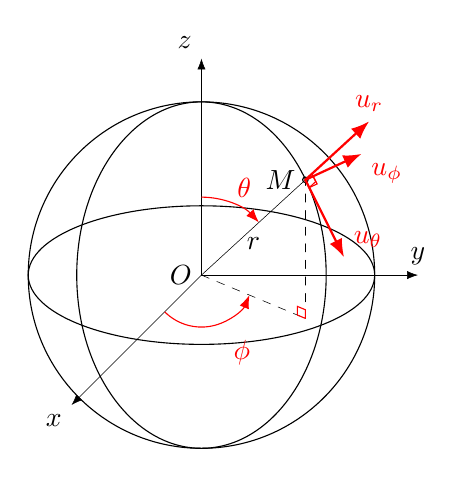
\begin{tikzpicture}[>=Latex,scale=1.1]
%\tkzDefPoint(0,0){O} ;
%\tkzDefPoint(-1,-1){x} ;
%\tkzDefPoint(2,0){y} ;
%\tkzDefPoint(0,2){z} ;
%\tkzLabelPoints[left](O) ;
%\tkzLabelPoints[below left](x) ;
%\tkzLabelPoints[above](y) ;
%\tkzLabelPoints[above left](z) ;

\tkzDefPoint[label={left:$O$}](0,0){O}
\tkzDefPoint[label={below left:$\vv x$}](-1.5,-1.5){vx}
\tkzDefPoint[label={above:$\vv y$}](2.5,0){vy}
\tkzDefPoint[label={above left:$\vv z$}](0,2.5){vz}
\tkzDrawSegment[->](O,vx) ;
\tkzDrawSegment[->](O,vy);
\tkzDrawSegment[->](O,vz);

\tkzDefPoint(1.2,1.1){M} ;
\tkzDrawPoint(M);
\tkzDrawSegment(O,M) ;
\tkzLabelPoints[left](M) ;
\tkzDefPoint(1.2,-0.5){M'} ;
\tkzDrawSegment[dashed](O,M') ;
%\tkzLabelPoints[below right](M') ;

\draw[thin] (0,0) [elliparc=0:360:2.0cm and .8cm];
\draw[thin] (0,0) [elliparc=0:360:1.44cm and 2.0cm];
\draw[thin] (0,0) [elliparc=0:360:2.0cm and 2.0cm];

%\tkzDefPointBy[translation=from O to vy](M') \tkzGetPoint{xM1}
%\tkzInterLL(O,vx)(M',xM1) \tkzGetPoint{xM}
%\tkzDefPointBy[translation=from O to vx](M') \tkzGetPoint{yM1}
%\tkzInterLL(O,vy)(M',yM1) \tkzGetPoint{yM}

\tkzDefPointBy[translation=from O to M'](M) \tkzGetPoint{zM1}
\tkzInterLL(O,vz)(M,zM1) \tkzGetPoint{zM}

%\tkzLabelPoint[below right](xM){$x$} ;
%\tkzLabelPoint[above ](yM){$y$} ;
%\tkzLabelPoint[above left](zM){$z$} ;
%\tkzDrawSegment[dashed](M',xM) ;
%\tkzDrawSegment[dashed](M',yM) ;
%\tkzDrawSegment[dashed](M,zM) ;
%\tkzLabelSegment[above,pos=.5](M,zM){$r$}
\tkzLabelSegment[below,pos=.5](O,M){$r$}
\tkzDrawSegment[dashed](M',M) ;
\tkzMarkAngle[mark=none,size=.6cm,->,color=red](vx,O,M') ;
\tkzLabelAngle[color=red,xshift=.3cm,yshift=.1cm](vx,O,M'){$\phi$} ;
\tkzMarkAngle[mark=none,size=.9cm,<-,color=red](M,O,vz) ;
\tkzLabelAngle[color=red,xshift=.1cm,yshift=.1cm](M,O,vz){$\theta$} ;

\tkzDefPointWith[linear,K=2](O,M) \tkzGetPoint{M2}
\tkzDefPointWith[linear normed](M,M2) \tkzGetPoint{ur}
\tkzDefPoint(1.85,1.4){phi} ;
\tkzDefPointWith[linear](M,phi) \tkzGetPoint{uphi}
\tkzDefPoint(1.4,0.7){theta} ;
\tkzDefPointWith[linear normed](M,theta) \tkzGetPoint{utheta}
\tkzDrawSegment[red,->,thick](M,ur);
\tkzDrawSegment[red,->,thick](M,utheta) ;
\tkzDrawSegment[red,->,thick](M,uphi) ;
\tkzLabelPoint[above, red](ur){$\vv u_r$} ;
\tkzLabelPoint[above right, red](utheta){$\vv u_\theta$} ;
\tkzLabelPoint[below right, red](uphi){$\vv u_\phi$} ;

\tkzMarkRightAngle[,size=.1,color=red](O,M',M);
\tkzMarkRightAngle[,size=.1,color=red](ur,M,utheta);
\tkzMarkRightAngle[,size=.1,color=red](uphi,M,utheta);
\end{tikzpicture}
\end{minipage}

\end{boite}

\section{Accélération d'un point}

En cinématique, l'accélération peut être définie comme est une grandeur qui mesure pour un mouvement, le rapport de la variation de vitesse de l'objet en fonction du temps.\\

Soit $M$ la position d'un mobile à un instant $t$. Soit $R$ un référentiel et $O$ un point fixe de ce référentiel.\\
On note $\vv \gamma(M_{/R})$ le vecteur accélération du mobile par rapport au référentiel $R$.\\
On peut exprimer alors cette accélération :
\begin{align*}
    &\vv \gamma(M_{/R})=\left(\frac{d(\vv v(M_{/R}))}{dt}\right)_{/R}\\
    &\tikz[baseline]{
        \node[fill=red!20,anchor=base,rounded corners]
        {$\vv \gamma(M_{/R})=\left(\dfrac{d^2(\vv{OM})}{dt^2}\right)_{/R}$};
    } 
\end{align*}

Comme dans le cas de la vitesse, le référentiel par rapport auquel nous calculerons l'accélération sera, sauf mention contraire, celui associé aux coordonnées cartésiennes. \\
Dans ce référentiel $R_c$, l'origine $O$ ainsi que la base ($\vv u_x$, $\vv u_y$, $\vv u_z$) sont fixes.

\begin{boite}[Expression de ll'accélération en coordonnées cartésiennes]
Soit ($\vv u_x$, $\vv u_y$, $\vv u_z$) la base des coordonnées cartésiennes.
\begin{align*}
    &\vv \gamma(M_{/R_c})=\left(\frac{d^2(\vv{OM})}{dt^2}\right)_{/R_c} \ \ \text{avec} \ \ \vv{OM} = x \vv u_x + y \vv u_y + z \vv u_z\\
        &\tikz[baseline]{
            \node[fill=red!20,anchor=base,rounded corners]
            {$\vv \gamma(M_{/R_c})=\dfrac{d^2x}{dt^2}\vv u_x + \dfrac{d^2y}{dt^2}\vv u_y + \dfrac{d^2z}{dt^2}\vv u_z$};
        } 
\end{align*}
On applique la même méthode de calcul que pour la vitesse.

\end{boite}

\begin{boite}[Expression de l'accélération en coordonnées polaires]
L'accélération est ici calculée par rapport au référentiel associé aux coordonnées cartésiennes.\\
Elle s'exprime sur la base des coordonnées polaires ($\vv u_r$, $\vv u_\theta$).\\

\begin{flalign*}
    &\vv \gamma(M_{/R_c})=\left(\frac{d^2(\vv{OM})}{dt^2}\right)_{/R_c} =\left(\frac{d(\vv v(M_{/R_c}))}{dt}\right)_{/R_c} \ \ \text{avec} \ \ \vv v(M_{/R_c})=\dfrac{dr}{dt}\vv u_r + r\dfrac{d\theta}{dt}\vv u_\theta&\\
    &\vv \gamma(M_{/R_c})=\left(\frac{d(\dfrac{dr}{dt}\vv u_r + r\dfrac{d\theta}{dt}\vv u_\theta)}{dt}\right)_{/R_c}\\
    &\tikz[baseline]{
            \node[fill=red!20,anchor=base,rounded corners]
            {$\vv \gamma(M_{/R_c})=\left(\dfrac{d^2r}{dt^2}-r\left(\dfrac{d\theta}{dt}\right)\right)\vv u_r + \left(2\dfrac{dr}{dt}\dfrac{d\theta}{dt}+\dfrac{d^2\theta}{dt^2}\right)\vv u_\theta$};
        } 
\end{flalign*}
\end{boite}


\begin{boite}[Expression de l'accélération en coordonnées cylindriques]
L'accélération est ici calculée par rapport au référentiel associé aux coordonnées cartésiennes.\\
Elle s'exprime sur la base des coordonnées cylindriques ($\vv u_r$, $\vv u_\theta$, $\vv u_z$).\\
\begin{minipage}{.63\textwidth}
\begin{flalign*}
    &\vv \gamma(M_{/R_c})=\left(\frac{d^2(\vv{OM})}{dt^2}\right)_{/R_c}\ \ \text{avec} \ \ \vv{OM} = r \vv u_r + z \vv u_z&\\
    &\vv \gamma(M_{/R_c})=\left(\frac{d(\dfrac{dr}{dt}\vv u_r + r\dfrac{d\theta}{dt}\vv u_\theta + z \vv u_z)}{dt}\right)_{/R_c}\\
    &\tikz[baseline]{
            \node[fill=red!20,anchor=base,rounded corners]
            {$\vv \gamma(M_{/R_c})=\left(\dfrac{d^2r}{dt^2}-r\left(\dfrac{d\theta}{dt}\right)\right)\vv u_r + \left(2\dfrac{dr}{dt}\dfrac{d\theta}{dt}+\dfrac{d^2\theta}{dt^2}\right)\vv u_\theta + \dfrac{d^2z}{dt^2}\vv u_z$};
        } 
\end{flalign*}
\end{minipage}
\hfill
\begin{minipage}{.35\textwidth}
\begin{tikzpicture}[>=Latex,scale=1.3]
%\tkzDefPoint(0,0){O} ;
%\tkzDefPoint(-1,-1){x} ;
%\tkzDefPoint(2,0){y} ;
%\tkzDefPoint(0,2){z} ;
%\tkzLabelPoints[left](O) ;
%\tkzLabelPoints[below left](x) ;
%\tkzLabelPoints[above](y) ;
%\tkzLabelPoints[above left](z) ;

\tkzDefPoint[label={left:$O$}](0,0){O}
\tkzDefPoint[label={below left:$\vv x$}](-1,-1){vx}
\tkzDefPoint[label={above:$\vv y$}](2.3,0){vy}
\tkzDefPoint[label={above left:$\vv z$}](0,2){vz}
\tkzDrawSegment[->](O,vx) ;
\tkzDrawSegment[->](O,vy);
\tkzDrawSegment[->](O,vz);

\tkzDefPoint(1.2,1.1){M} ;
\tkzDrawPoint(M);
\tkzDrawSegment(O,M) ;
\tkzLabelPoints[below right](M) ;
\tkzDefPoint(1.2,-0.5){M'} ;
\tkzDrawSegment[dashed](O,M') ;
%\tkzLabelPoints[below right](M') ;

\draw[thin] (0,0) [elliparc=0:360:1.75cm and .7cm];
\draw[thin] (0,1.6) [elliparc=0:360:1.75cm and .7cm];

%\tkzDefPointBy[translation=from O to vy](M') \tkzGetPoint{xM1}
%\tkzInterLL(O,vx)(M',xM1) \tkzGetPoint{xM}
%\tkzDefPointBy[translation=from O to vx](M') \tkzGetPoint{yM1}
%\tkzInterLL(O,vy)(M',yM1) \tkzGetPoint{yM}

\tkzDefPointBy[translation=from O to M'](M) \tkzGetPoint{zM1}
\tkzInterLL(O,vz)(M,zM1) \tkzGetPoint{zM}

%\tkzLabelPoint[below right](xM){$x$} ;
%\tkzLabelPoint[above ](yM){$y$} ;
%\tkzLabelPoint[above left](zM){$z$} ;
%\tkzDrawSegment[dashed](M',xM) ;
%\tkzDrawSegment[dashed](M',yM) ;
\tkzDrawSegment[dashed](M,zM) ;
\tkzLabelSegment[above,pos=.5](M,zM){$r$}
\tkzLabelSegment(O,zM){$z$}
\tkzDrawSegment[dashed](M',M) ;
\tkzMarkAngle[mark=none,size=.6cm,->,color=red](vx,O,M') ;
\tkzLabelAngle[color=red,xshift=.3cm,yshift=.1cm](vx,O,M'){$\theta$} ;

\tkzDefPointWith[linear,K=2](zM,M) \tkzGetPoint{M2}
\tkzDefPointWith[linear normed](M,M2) \tkzGetPoint{ur}
\tkzDefPointWith[colinear normed= at M](M',yM) \tkzGetPoint{utheta}
\tkzDefPointWith[colinear normed= at M](O,zM) \tkzGetPoint{uz}
\tkzDrawSegment[red,->,thick](M,ur);
\tkzDrawSegment[red,->,thick](M,utheta) ;
\tkzDrawSegment[red,->,thick](M,uz) ;
\tkzLabelPoint[below right, red](ur){$\vv u_r$} ;
\tkzLabelPoint[above, red](utheta){$\vv u_\theta$} ;
\tkzLabelPoint[above, red](uz){$\vv u_z$} ;

\tkzMarkRightAngle[,size=.1,color=red](O,M',M);
\tkzMarkRightAngle[,size=.1,color=red](O,zM,M);
\tkzMarkRightAngle[,size=.1,color=red](ur,M,utheta);
\tkzMarkRightAngle[,size=.1,color=red](uz,M,utheta);

\end{tikzpicture}
\end{minipage}

\end{boite}

\end{document}